\section{Dynamic motion analysis}
    \subsection{Constant driving force/torque}
        \subsubsection{Velocity and Acceleration}
            Providing a constant input torque of 5500 kg-mm\^2/s\^2 clockwise.
            \begin{enumerate}
                \item 
                    \begin{figure}[hbt!]
                        \centering
                        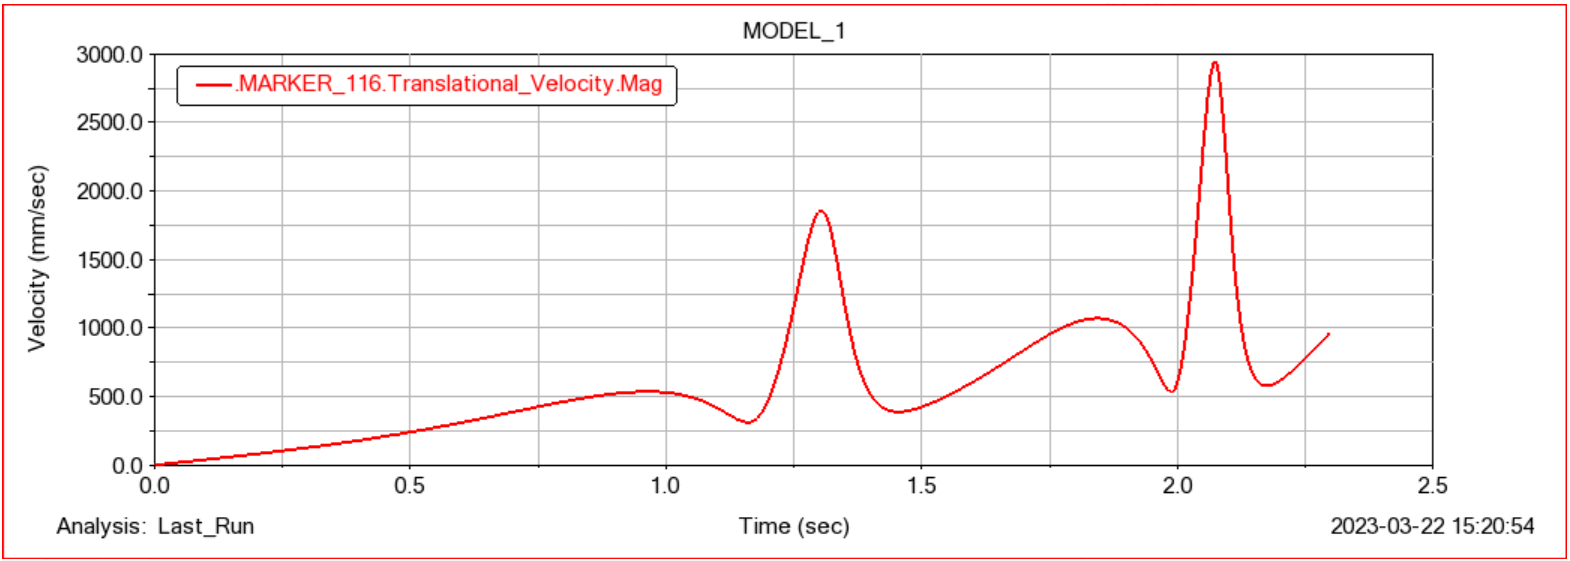
\includegraphics[width=0.9\columnwidth]{Images/Velocity_311.png}
                        \caption{Velocity vs time}
                        \label{fig:vel_1}
                    \end{figure}
                    Velocity plot is shown in fig~\ref{fig:vel_1}
                \item 
                    \begin{figure}[hbt!]
                        \centering
                        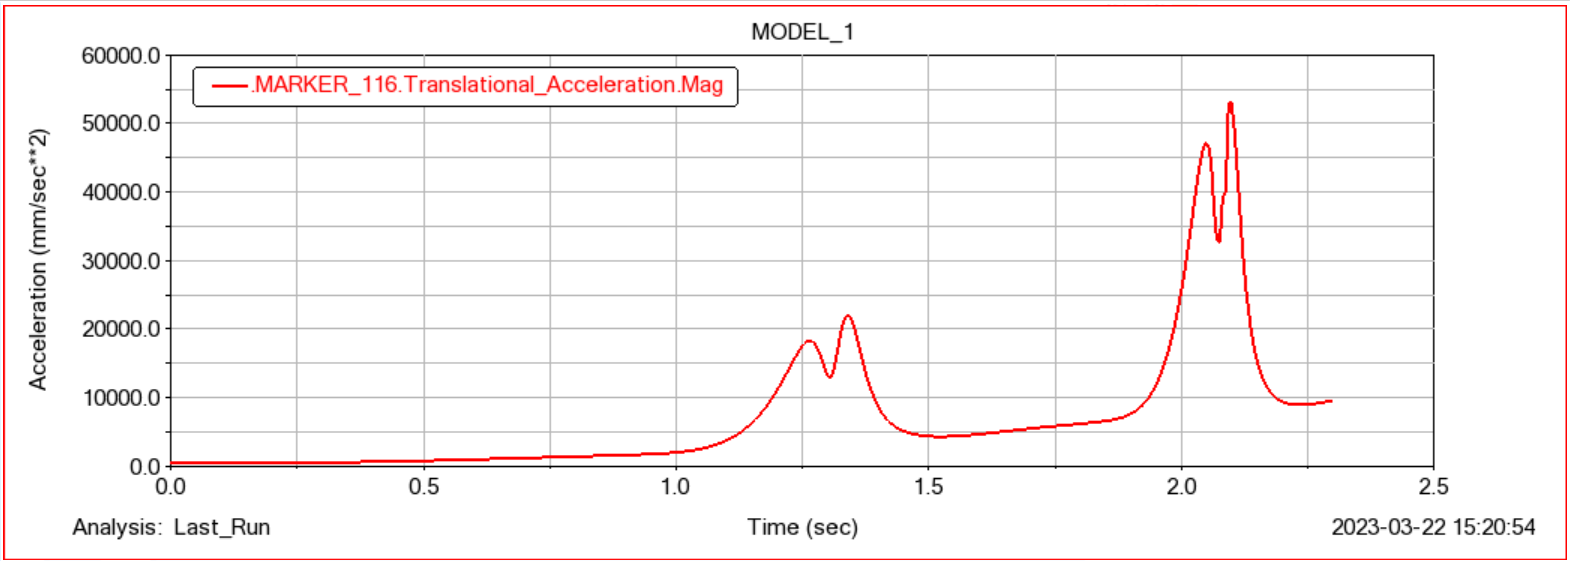
\includegraphics[width=0.9\columnwidth]{Images/Acceleration_311.png}
                        \caption{Acceleration vs time}
                        \label{fig:acc_1}
                    \end{figure}
                    Acceleration plot is shown in fig~\ref{fig:acc_1}
            \end{enumerate}
        \subsubsection{Sub2}
            Applying twice the torque applied in previous section i.e. -11000 kg-mm\^2/s\^2. Superimposed plots are shown below.
            \begin{enumerate}
                \item 
                    \begin{figure}[hbt!]
                        \centering
                        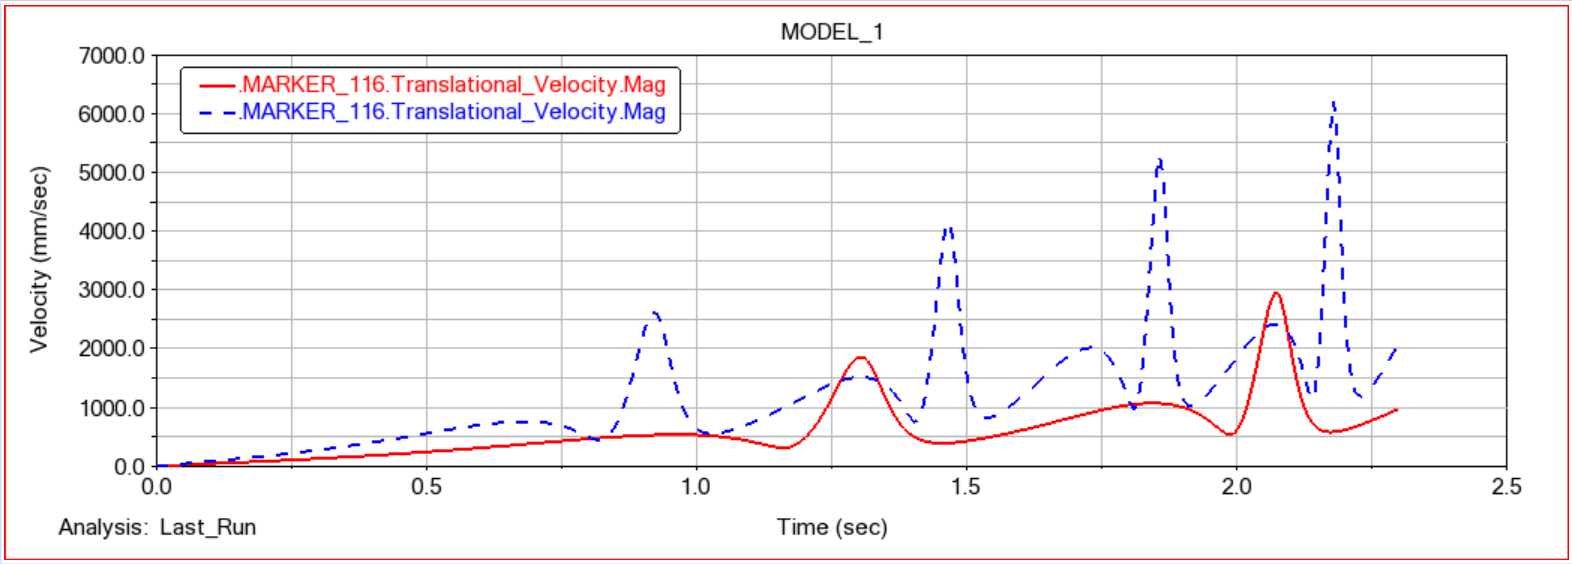
\includegraphics[width=0.9\columnwidth]{Images/Velocity_312.png}
                        \caption{Superimposed velocity vs time}
                        \label{fig:vel_2}
                    \end{figure}
                    Velocity plot is show in fig~\ref{fig:vel_2}
                \item 
                    \begin{figure}[hbt!]
                        \centering
                        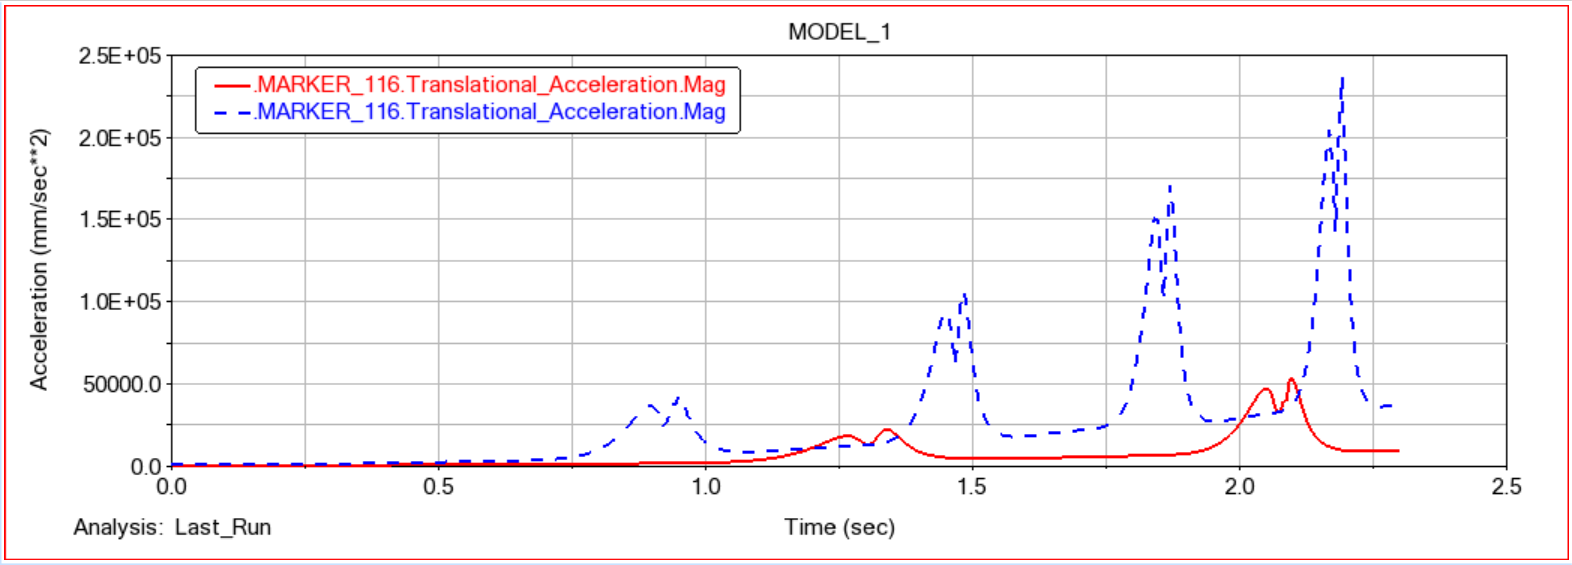
\includegraphics[width=0.9\columnwidth]{Images/Acceleration_312.png}
                        \caption{Superimposed acceleration vs time}
                        \label{fig:acc_2}
                    \end{figure}
                    Acceleration plot is shown in fig~\ref{fig:acc_2}
            \end{enumerate}
            
    \subsection{Sinusoidal driving force/torque}
        Now we apply sinusoidal torque $T = 1.4*5500*(1+\sin(40t))$.
        \begin{figure}[hbt!]
            \centering
            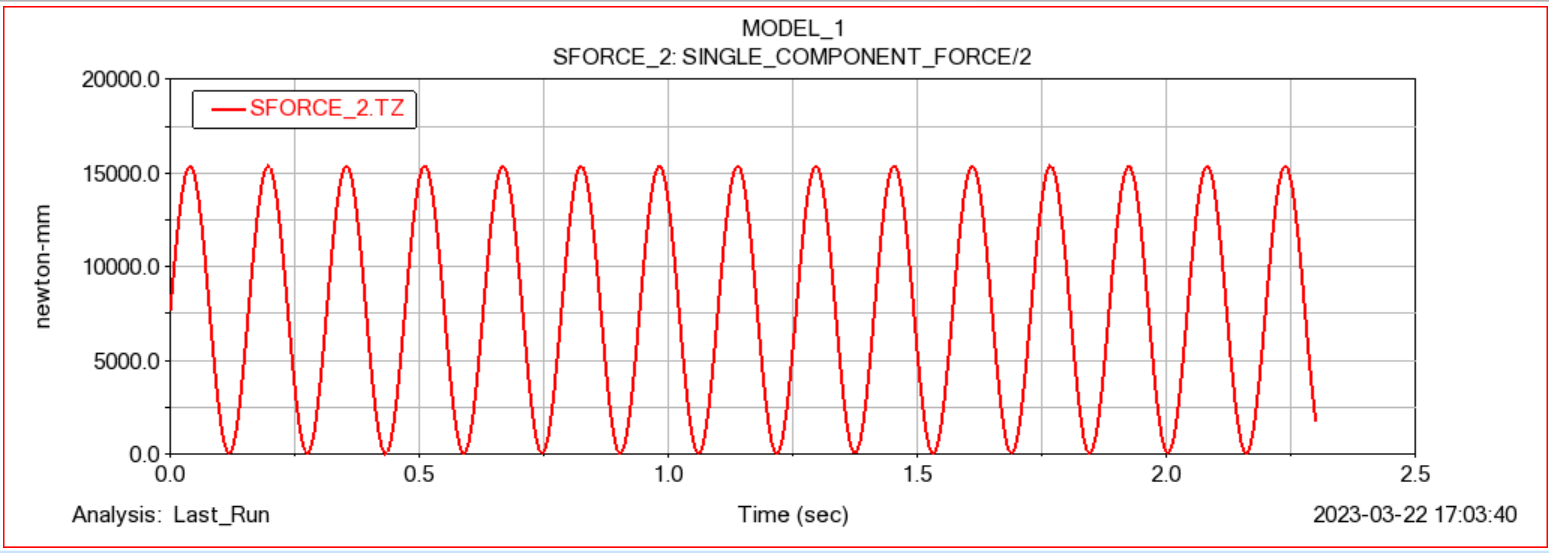
\includegraphics[width=0.9\columnwidth]{Images/Force_sinusoidal.png}
            \caption{Sinusoidal force vs time}
            \label{fig:sin_force}
        \end{figure}
        The force graph has been shown in fig~\ref{fig:sin_force}.
        \begin{enumerate}
            \item 
                \begin{figure}[hbt!]
                    \centering
                    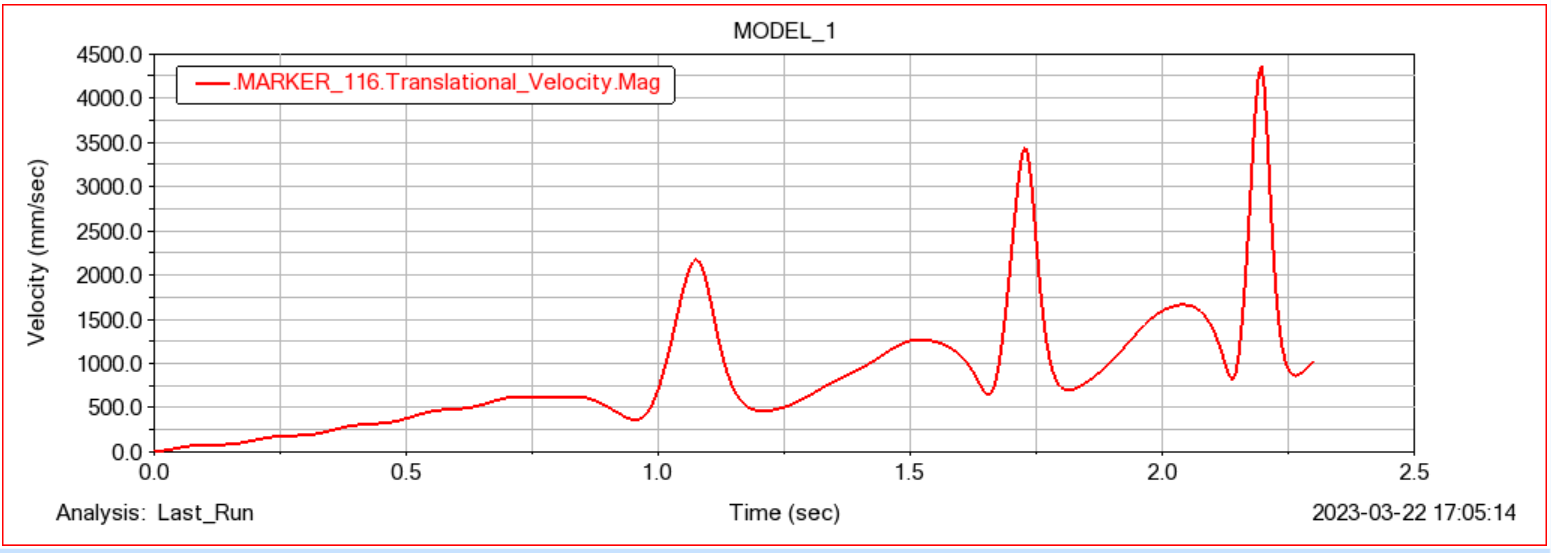
\includegraphics[width=0.9\columnwidth]{Images/sine_vel.png}
                    \caption{Velocity for sine force vs time}
                    \label{fig:sine_vel}
                \end{figure}
                Velocity plot is shown in fig~\ref{fig:sine_vel}
            \item 
                \begin{figure}[hbt!]
                    \centering
                    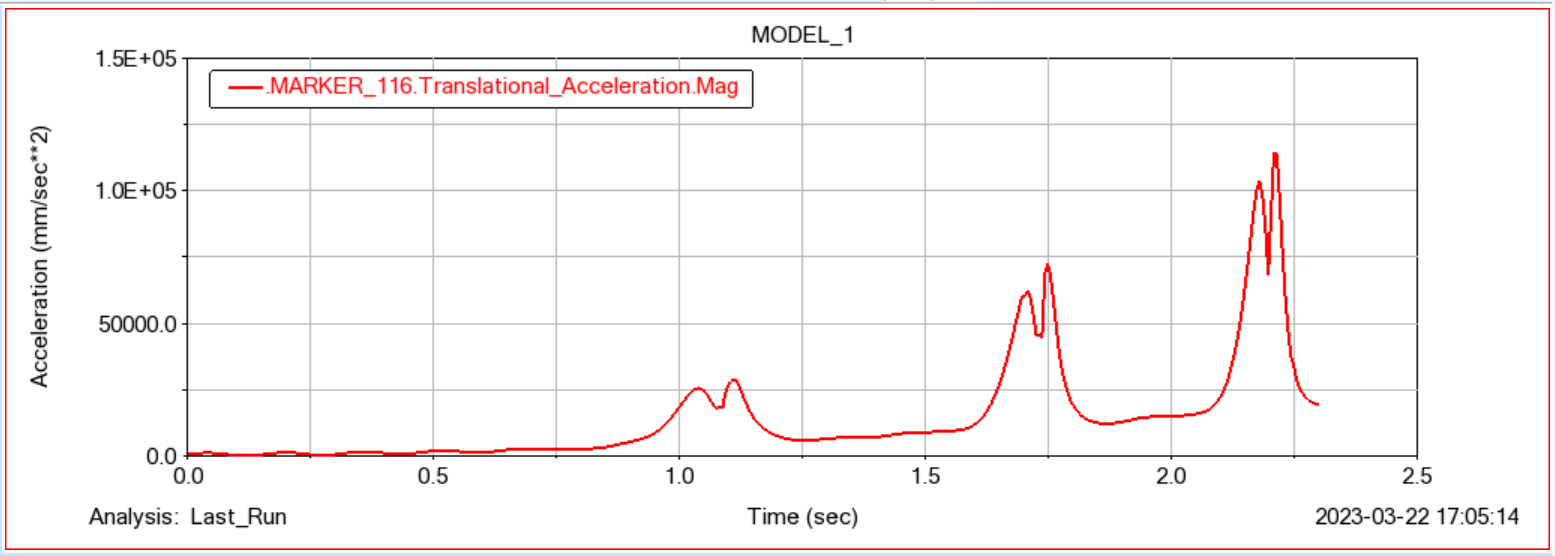
\includegraphics[width=0.9\columnwidth]{Images/sine_acc.png}
                    \caption{Acceleration for sine force vs time}
                    \label{fig:sine_acc}
                \end{figure}
                Acceleration plot is shown in fig~\ref{fig:sine_acc}
        \end{enumerate}